\textit{Le but de ce TP est d'implémenter deux algorithmes de résolution du problème de flot maximum : l'algorithme d'Edmonds-Karp et l'algorithme de Dinic. Nous commencerons par spécifier les fonctionnalités que devra implémenter notre programme, puis nous détaillerons la manière dont ces fonctionnalités ont été développées. Une troisième partie sera consacrée aux tests effectués sur les deux algorithmes ainsi qu'à l'analyse des résultats.}

\section{Spécifications fonctionnelles}

\subsection{Résolution du problème de flot maximum}

Le programme doit être capable de :
\begin{itemize}
\item générer et d'actualiser les graphes d'écarts successifs
\item calculer la valeur du flot obtenu à partir du graphe d'écart final
\item résoudre le problème de flot maximum en suivant l'algorithme d'\textbf{Edmonds-Karp}
\item résoudre le problème de flot maximum en suivant l'algorithme de \textbf{Dinic}
\item retourner la solution de manière exploitable pour l'analyse
\end{itemize}

Il faudra veiller à conserver la complexité des deux algorithmes, notamment en prenant garde aux structures de données et librairies utilisées.

\subsection{Génération aléatoire d'un réseau de transport}

La génération aléatoire de graphes de type réseau de transport permettra de tester les deux algorithmes. Il faudra veiller à ce que le graphe respecte les conditions d'un réseau de transport notamment la possession d'une source et d'un puits, la pondération des arcs (capacités), et assurer la connexité du graphe. La génération de ce réseau de transport devra être paramétrable selon la taille (nombre de sommets) et la densité (nombre d'arcs).

La densité du graphe correspond à son taux d'arêtes par rapport au nombre d'arêtes du graphe complet non orienté ayant le même nombre de sommets. Soit la formule suivante :
\[ \textsl{nb\_aretes} = \frac{n*(n-1)}{2}*\textsl{taux}\]

\section{Spécifications techniques}

\subsection{Langage de programmation et organisation}

\subsubsection{Programmation C++}
En plus de sa notoriété, nous avons choisi de développer l'application en C++ car il s'agit d'un bon compromis entre langage orienté objet et langage de bas niveau. Nous pourrons ainsi abstraire la gestion des graphes (notamment des structures de données) dans nos algorithmes, tout en gardant la possibilité d'optimiser le code grâce à la flexibilité du langage C++.

\subsubsection{Utilisation d'un gestionnaire de version}
Nous avons d'utilisés un gestionnaire de version afin de pouvoir sauvegarder et partager notre code entre les membres
de l'équipe.	

\subsection{Représentation du problème de flot maximum}

Le problème du flot maximum n'est défini que pour un certain type de graphes appelé \emph{réseau de transport}.

\subsubsection{Réseau de transport}
Les réseaux de transport peuvent êtres représenté par un graphe orienté pondéré pour lequel on défini un sommet
source et un sommet puits. Le sommet source à la particularité de ne pas avoir de prédecesseur et le puits celui
de ne pas avoir de successeur. La valuation d'un arcs représente sa capacité maximal.

\subsubsection{Graphe d'écart}
Les graphes d'écart peuvent êtres simplement représenté par un graphe orienté pondéré.

\subsubsection{Graphe de couches}
Les graphes de couches peuvent êtres représenté par un graphe orienté pondéré auquel on ajoute un tableau 
de listes de sommets indexé par le numéro de couche. Chaque liste représente donc une couche du graphe, elle contient donc l'ensemble des sommets se trouvant à une distance d du graphe où d est le numéro de la couche.


\subsection{Modélisation}

\subsubsection{Diagramme de classes}

Afin de s'abstraire de la structure de donnée, nous avons choisi de créer une classe abstraite \texttt{AbstractGraph} dont deux classes fille héritent. Un graphe peut donc être de type \texttt{AdjacencyListGraph} ou \texttt{MatrixGraph}. Cela permet une grande généricité des algorithme développés, ce qui permet d'utiliser une structure de données de manière totalement détachée des algorithmes.
\begin{figure}[t]
\begin{center}
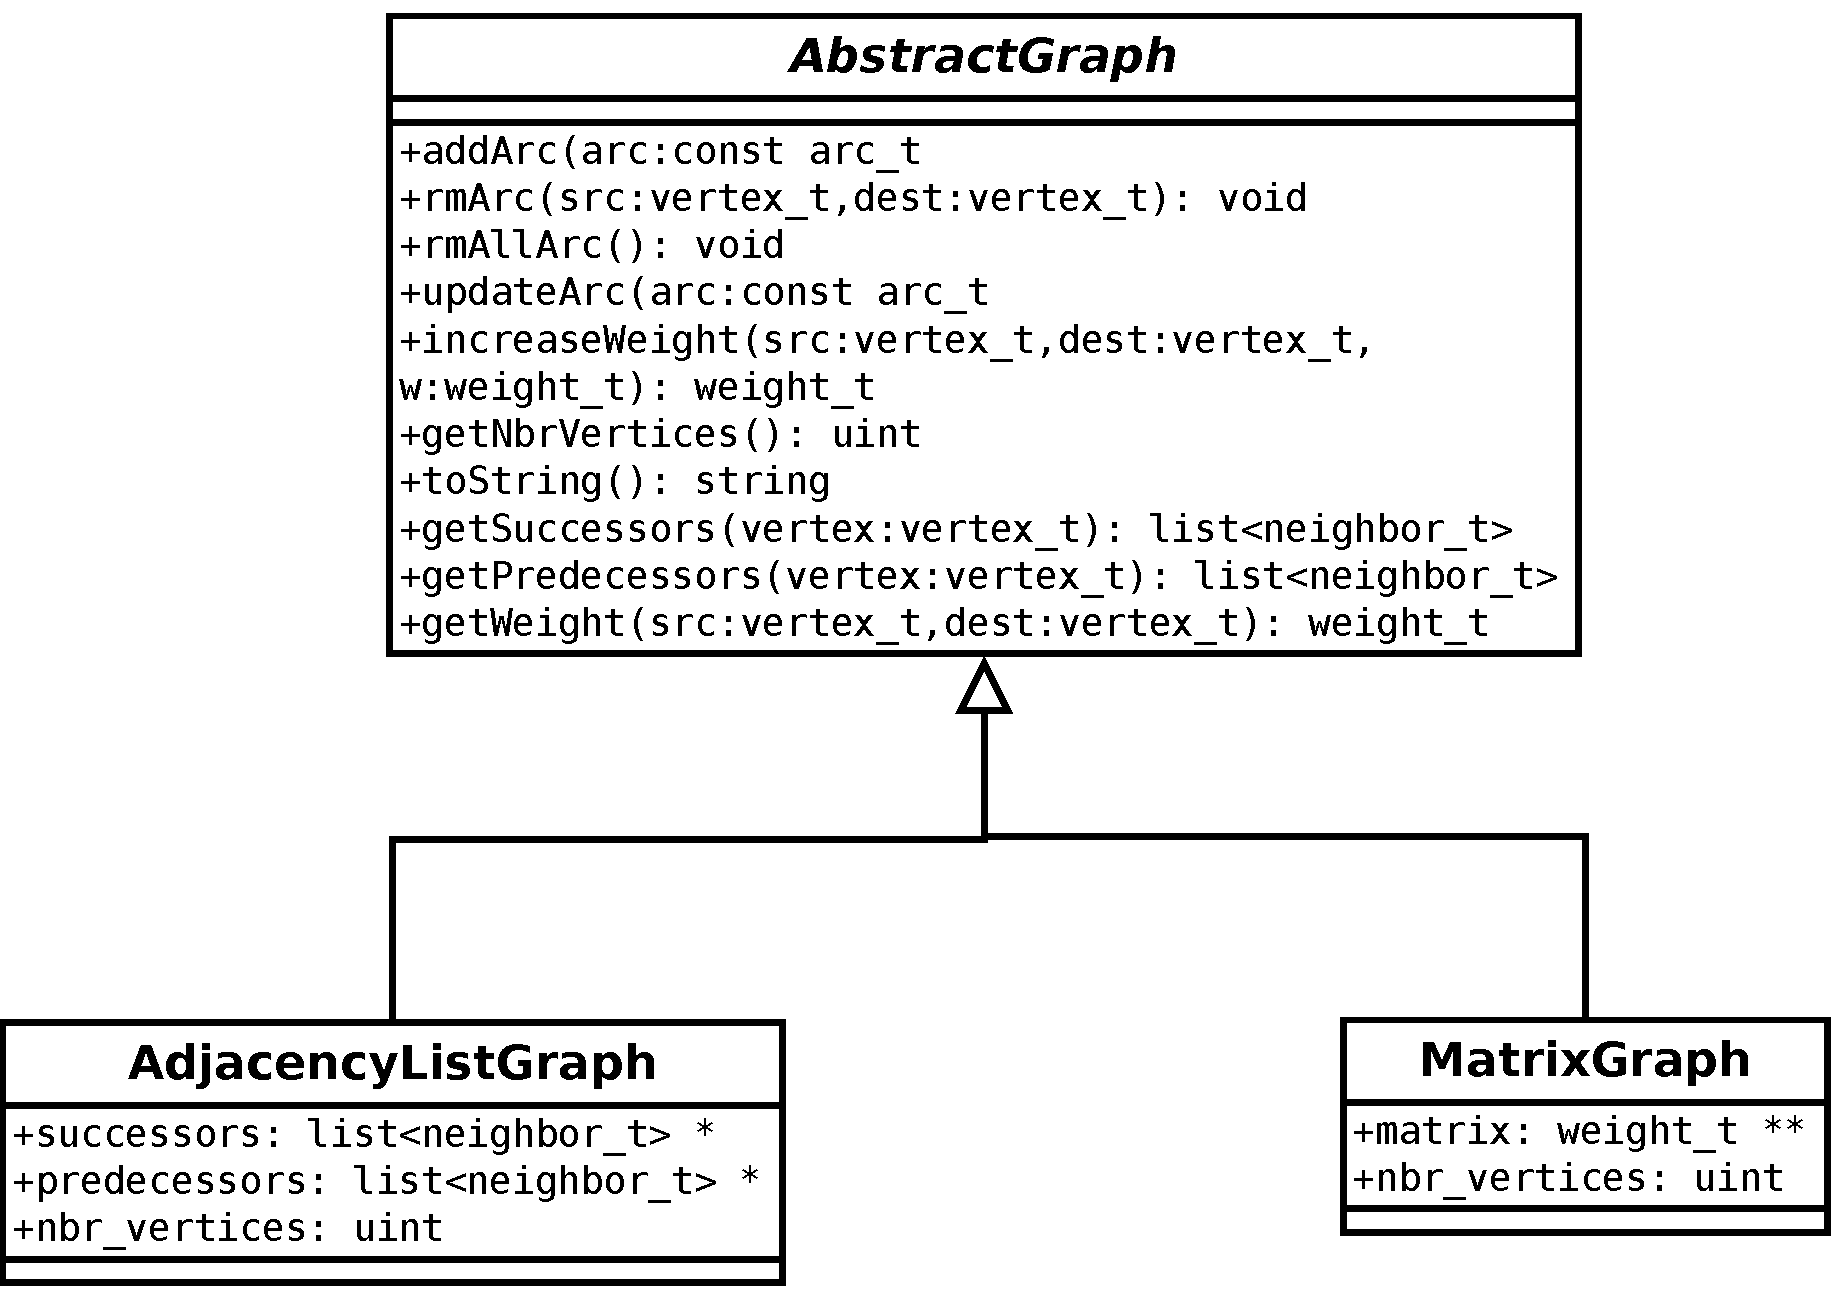
\includegraphics[width=\textwidth]{files/diag_class}
\end{center}
\caption{Diagramme de classes.}
\end{figure}

\FloatBarrier

Les graphes peuvent être stockés à l'aide différents types de structures de données. Nous avons choisi d'en implémenter deux :  par listes d'adjacences et par matrice d'adjacences.
\begin{description}
\item[Listes d'adjacences] : chaque sommet possède la liste de ses voisins. Ces listes ont l'avantage d'allouer de la mémoire uniquement lorsqu'une information doit être stockée. 
\item[Matrice d'adjacences] : la mémoire allouée pour cette structure de données ne dépend que du nombre de sommets ($n^2$). Cette structure a l'avantage d'offrir un accès direct à un arc pour deux sommets donnés.
\end{description}

Dans un but d'optimisation mémoire, on utilise en général des listes d'adjacences lorsque l'on travail sur des graphes peu denses. En effet, la taille allouée par cette structure de données étant directement dépendante du nombre d'arcs, elle est donc réduite par rapport aux matrices d'adjacences. Sur des graphes très dense, on utilisera en revanche des matrices d'adjacences, permettant un accès aux données plus rapide. 

Les ressources matériels disponibles peuvent également orienter ce choix.

\subsubsection{Application aux réseaux de transport}
Les deux classe précédentes n'étant pas spécialisées dans la modélisation de réseaux de transport, nous adopterons les conventions suivantes :
\begin{itemize}
\item le sommet zéro (premier sommet) représente la source,
\item le sommet n (dernier sommet) représente le puits,
\item la pondération affecté à chaque arc représente sa capacité.
\end{itemize}

\subsection{Types et structures}

Déclaration des types \texttt{weight\_t}, \texttt{vertex\_t} et \texttt{path\_t}, et des structures \texttt{edge}, \texttt{neighbor\_t}

\lstinputlisting[language=C++,morekeywords={}]{./sources/structs}

\subsubsection{Classe \texttt{AbstractGraph}}

Cette classe permet une abstraction des différentes représentations d'un graphe (structures de données utilisées). Elle déclare les méthodes qui doivent êtres implémentées dans les classes filles.

Header de la classe \texttt{AbstractGraph}

\lstinputlisting[language=C++,morekeywords={}]{./sources/AbstractGraph}

\subsubsection{Classe \texttt{AdjacencyListGraph}}
Cette classe représente un orienté valué sous la forme
de deux listes d'adjacences : une représente les 
successeurs d'un sommet, l'autre les prédécesseurs.

Ce doublon d'information permet d'accélérer l'accès aux voisins d'un sommet, notamment à ces prédécesseurs. En effet, cette méthode nous permet d'accéder à une liste des prédécesseurs directement (complexité de $O(1)$) alors que l'accès via les listes des successeurs implique le parcours de toutes ces listes (complexité de $O(nm)$).

Ces doubles listes d'adjacences nous assurent un gain de performances en terme de rapidité, qui se fait au détriment de la quantité de mémoire utilisé, qui se trouve doublée.

Header de la classe \texttt{AdjacencyListGraph}

\lstinputlisting[language=C++,morekeywords={}]{./sources/AdjacencyListGraph}


\subsubsection{Classe \texttt{MatrixGraph}}

Cette classe représente un graphe orienté valué sous la forme d'une matrice d'adjacence. L'absence d'un arc est représenté par la valeur $-1$. Toute valeur positive représente la pondération de l'arc.

Header de la classe \texttt{MatrixGraph}

\lstinputlisting[language=C++,morekeywords={}]{./sources/MatrixGraph}


\section{Génération aléatoire de réseaux de transport}

\subsection{Stratégies de génération des arcs}

La première stratégie utilisée par notre application était naïve. Nous commencions par tracer un chemin de la source vers le puits pour s'assurer de la connexité du graphe. Puis on ajoutait aléatoirement des arcs.

\begin{algorithm}[H]
  \caption{flowNetworkGenerator1(G,rate,min\_weight,max\_weight)}
  \Donnees{\\
    G \textit{// Graphe d'entrée}\\
    rate \textit{// Densité}\\
    min\_weight \textit{// Capacité minimum}\\
    max\_weight \textit{// Capacité maximum}
  }
  \Deb{
  nb\_vertices $\leftarrow$ G.getNbrVertices()\;
  nb\_arcs $\leftarrow$ nbr\_arcs\_max(nbr\_vertices)*rate\;
  
  \textit{//génération d'un chemin}\\
  \Pour{$u$ allant de 1 à $(nbr\_vertices - 1$}{
    weight $\leftarrow$ rand(min\_weight, max\_weight)\;
    g.add($u-1$, $u$)\;
    $- -$nb\_arcs\;
  }
  
  \textit{//génération des arcs}\\  
  \Tq{nb\_arcs$ > 0$}{
    $u \leftarrow$ rand \% (nb\_vertices - 1)\;
    $v \leftarrow$ (rand \% (nb\_vertices - 1)) + 1\;
    
    \Si{!G.contains($u,v$)}{
      weight $\leftarrow$ rand(min\_weight, max\_weight)\;
      G.add($u$,$v$,weight)\;
      $- -$nbr\_arcs\;
    }
  }
    \Retour G\;
  }
\end{algorithm}

Cet algorithme, bien que \og plutôt \fg fonctionnel pour des graphes peu denses ne fourni aucune garantie d'arrêt. Nous avons donc réfléchi à une deuxième approche, qui consistait à générer tout les arcs possibles dans un tableau de type vector puis de piocher parmi ces arcs.

\begin{algorithm}[H]
  \caption{flowNetworkGenerator(G,rate,min\_weight,max\_weight)}
  \Donnees{\\
    G \textit{// Graphe d'entrée}\\
    rate \textit{// Densité}\\
    min\_weight \textit{// Capacité minimum}\\
    max\_weight \textit{// Capacité maximum}
  }
  \Deb{
  nb\_vertices $\leftarrow$ G.getNbrVertices()\;
  nb\_arcs $\leftarrow$ nbr\_arcs\_max(nbr\_vertices)*rate\;
  vector$<$edge$>$vector\;
  edge e\;
  
 \textit{//génération de tous les arcs possibles}\\  
  \Pour{ $u$ allant de 1 à $(nbr\_vertices - 1$}{
    \textit{//Pour tout u, on crée l'arc u, u+1 afin d'assurer l’existence}\\
    \textit{//d'un chemin entre la source et le puits}
    G.addArc($u$,$u+1$,rand(min\_weight, max\_weight))\;
    $- -$nb\_arcs\;
    
    \Pour{$v$ allant de $u + 2$ à nb\_vertices$-1$}{
      e.u $\leftarrow$ $u$\;
      e.v $\leftarrow$ $v$\;
      vector.push\_back(e)\;
    }
  }
  
  \textit{//ajout des arcs}\\  
  \Tq{nb\_arcs$ > 0$}{
  index $\leftarrow$ rand() \% vector.size()\;
  \Tq{vector[index]$=$nil}{
  index $= ++$index \% vector.size()\;
  }
  
  e $\leftarrow$ vector.get(index)\;
  
  \Si{e.u $=0$ \textbf{OU} e.v $=$ nb\_vertices $-1$ \textbf{OU} rand() \% $2=1$}{
  	G.addArc(e.u,e.v,randMinMax(min\_weight,max\_weight)\;
  }
  \Sinon{
    G.addArc(e.v,e.u,randMinMax(min\_weight,max\_weight)\;
  }
  $- -$nb\_arcs\;
  vector[index]$=$nil\;
  }
    \Retour G\;
  }
\end{algorithm}

Dans tous les cas, nous sommes certain de l'arrêt de cet algorithme. Il faut veiller à utiliser un type tableau en marquant à \og nil \fg les arcs ajoutés. En effet, nous avions commencé par utiliser une liste chainée mais la fonction \texttt{list.get(...)} a une complexité en $O(n^2)$.


\subsection{Méthode implémentée}
Cette fonctionnalité est assurée par la fonction \texttt{flowNetworkGenerator} qui construit aléatoirement un réseau de transport sur le graphe passé en paramètre. Elle permet de spécifier le nombre de sommets, la densité du graphe et l'intervalle des capacités aléatoires.

Notons que cette méthode utilise la fonction \texttt{rand()} fournis par la librairie standard. Cette fonction \og pseudo-aléatoire \fg nécessite l'initialisation d'un générateur via la fonction \texttt{srand(int)}. Il est donc possible de sauvegarder la \og graine \fg, paramètre passée à la fonction \texttt{srand(int)}, afin de pouvoir régénérer un graphe identique.

Entête de la méthode de génération aléatoire de réseaux de transport
\lstinputlisting[language=C++,morekeywords={}]{./sources/aleatoire}

\section{Procédures principales}

\subsection{Algorithme d'Edmonds-Karp}

La méthode \texttt{edmondsKarp} permet l'exécution de cet algorithme. Il prend en paramètre par référence un réseau de transport.

Entête de la méthode d'exécution d'Edmonds-Karp
\lstinputlisting[language=C++,morekeywords={}]{./sources/ek}

La recherche du plus court chemin en nombre d'arc est implémenté par la fonction \texttt{leastArcsPath} qui effectue un parcours en largeur. Sa complexité est donc en $O(n+m)$ avec structure par listes d'adjacences, et en $O(n^2)$ par avec une structure par matrice d'adjacences.

La mise à jour du graphe d'écart est assurée par la méthode \texttt{updateResidualNetwork} avec une complexité en $O(n)$.

Entête des principales méthodes utilisées par la procédure \texttt{edmondsKarp}
\lstinputlisting[language=C++,morekeywords={}]{./sources/ek_methods}

\subsection{Algorithme de Dinic}

Entête de la méthode d'exécution de Dinic
\lstinputlisting[language=C++,morekeywords={}]{./sources/dinic}

Entête des principales méthodes utilisées par la procédure \texttt{dinic}
\lstinputlisting[language=C++,morekeywords={}]{./sources/dinic_methods}

\section{Tests \& résultats}

\subsection{Méthode de test}

\subsubsection{Série de tests}
Pour tester les performances des deux algorithmes implémentés, nous avons générer une série de problèmes à résoudre sur des réseaux de transports ayant les paramètres suivants :
\begin{itemize}
\item nombre de sommets variant de 100 à 1000 par palier de 100,
\item densité du graphe à 20\%, 50\% et 80\%,
\item capacité des arcs variant de 1 à 20.
\end{itemize}
Pour chaque test (un nombre de sommets et une densité donnés), nous avons généré 100 graphes afin de travailler sur des moyennes lors de l'analyse.

\subsubsection{GNU gprof}
Nous avons évalué les algorithmes en fonction de leurs temps d'exécution. Le temps réel d'exécution (real time) ayant peu de sens pour effectuer des statistiques correctes, nous avons choisi de mesurer les temps CPU (CPU time). Le temps CPU est le temps alloué au processus par le système d'exploitation sur le processeur. Contrairement au temps réel, le temps CPU est indépendant des autres processus en cours d'activité et aux interruptions systèmes : il s'agit du temps effectivement passé par le CPU pour traiter le processus.

L'analyse des temps CPU a été faite à l'aide de l'outil GNU gprof. Son utilisation requière l'ajout de l'argument \texttt{-pg} lors la compilation. A l'exécution du programme, un fichier \texttt{gmon.out} est généré. La commande \texttt{gprof} permet ensuite de créer un fichier texte de statistiques. Pour chaque méthode, un grand nombre de données sont disponibles, nous nous sommes intéressés principalement aux suivantes :
\begin{itemize}
\item pourcentage du temps CPU total,
\item temps CPU total,
\item temps CPU par appel, de manière cumulative (en prenant en compte les appel à d'autres fonctions) ou non.
\end{itemize}

\subsection{Analyse des résultats}

A partir des données obtenues, nous avons essayé de créer une série de graphiques ayant comme ordonnée le temps CPU, et en abscisse :
\begin{itemize}
  \item (1) le nombre de sommets (en conservant une densité identique),
  \item (2) la densité (en conservant un nombre d'arcs identique),
  \item (3) le nombre d'arcs (en faisant donc varier le nombre d'arc et la densité).
\end{itemize}

Seule la représentation (1) permet de mettre en évidence un phénomène intéressent. Ci-après sont donc présentés trois graphiques, pour des densités de 20\%, 50\% et 80\%.

\begin{figure}[h!]
\begin{center}
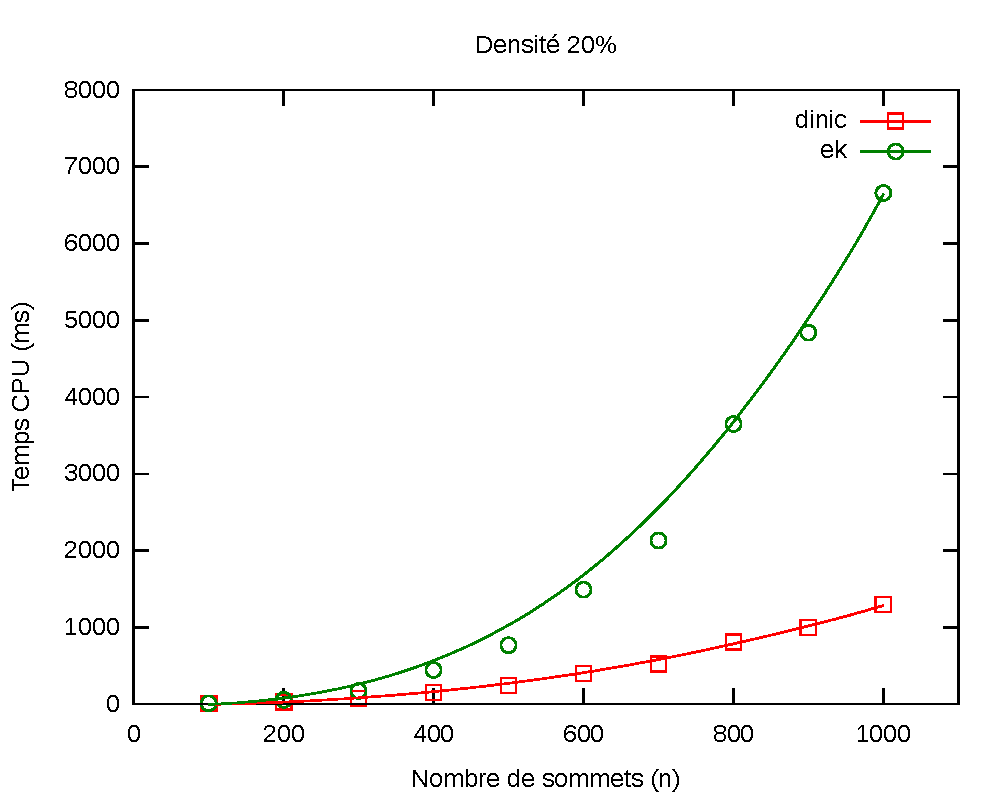
\includegraphics[width=\textwidth]{files/c20}
\end{center}
\caption{Temps CPU en fonction du nombre de sommets, densité de 20\%}
\end{figure}

\begin{figure}[h!]
\begin{center}
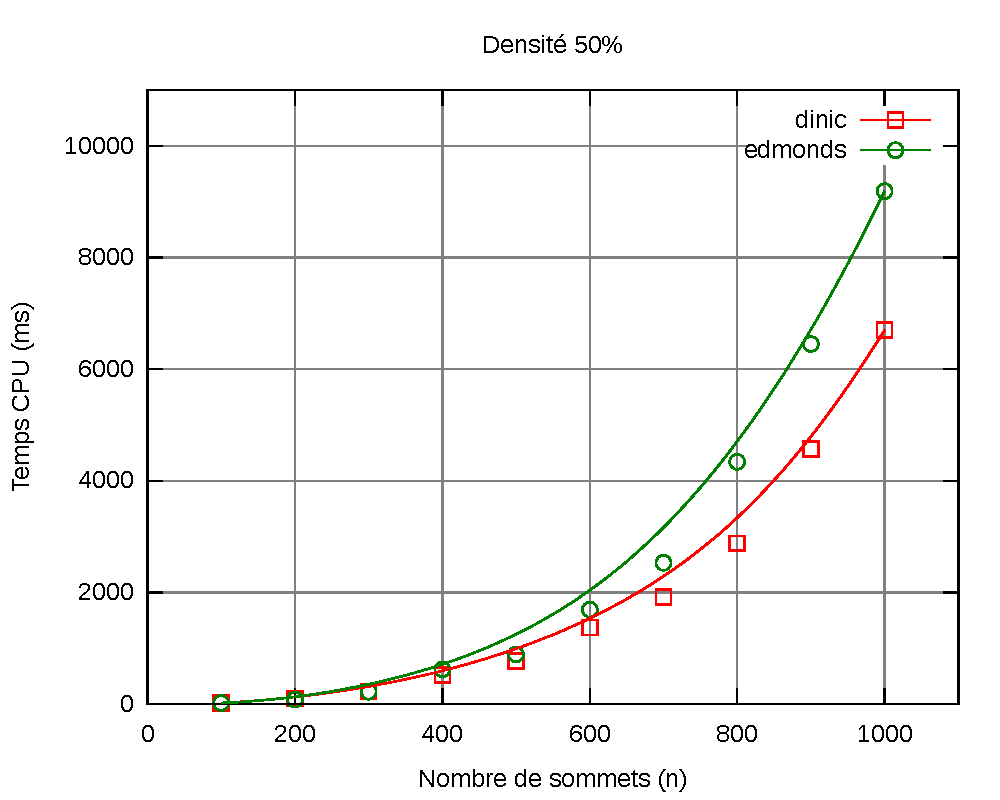
\includegraphics[width=\textwidth]{files/c50}
\end{center}
\caption{Temps CPU en fonction du nombre de sommets, densité de 50\%}
\end{figure}

\begin{figure}[h!]
\begin{center}
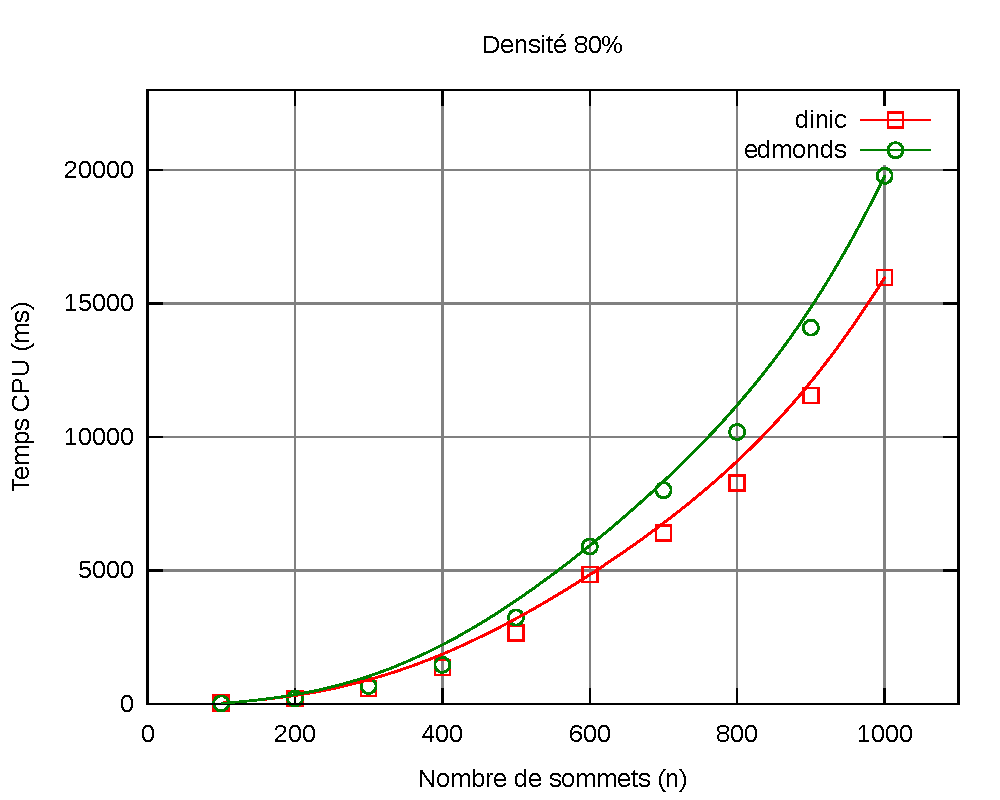
\includegraphics[width=\textwidth]{files/c80}
\end{center}
\caption{Temps CPU en fonction du nombre de sommets, densité de 80\%}
\end{figure}

\FloatBarrier

L'évolution du temps CPU de l'algorithme d'Edmonds-Karp change peu en fonction de la densité du graphe. Ces premiers graphiques montre également que l'algorithme de Dinic reste plus performant en terme de temps CPU même si l'on constate que l'écart diminue lorsque la densité augmente.

Ce résultat est cohérent, étant donné les complexité des algorithmes : 
\begin{itemize}
\item $O(nm^2)$ pour Dinic,
\item $O(n^ 2m)$ pour Edmonds-Karp,
\end{itemize}
il est normal que la densité influe plus sur le premier que le second.

Nous nous sommes cependant intéressés aux résultats obtenus sur des plus petits graphes. Voici deux graphiques qui montre nos résultats sur des graphes inférieurs à 200 sommets.

\begin{figure}[h!]
\begin{center}
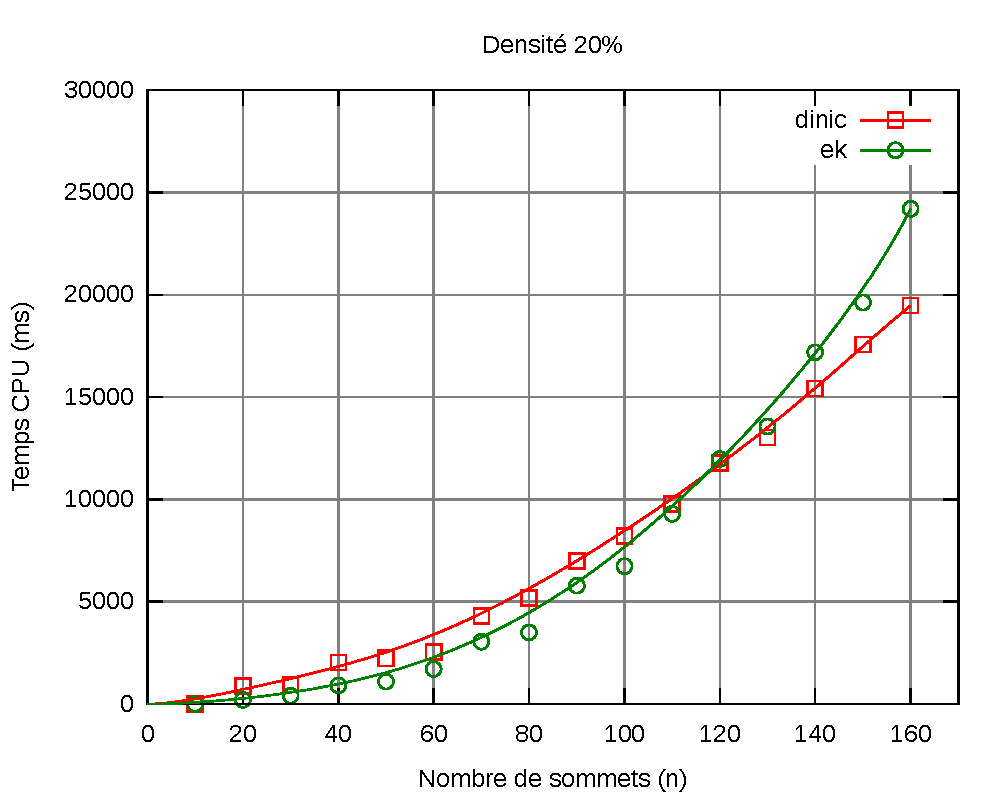
\includegraphics[width=\textwidth]{files/c20_low}
\end{center}
\caption{Temps CPU en fonction du nombre de sommets (valeur faible), densité de 20\%}
\end{figure}

\begin{figure}[h!]
\begin{center}
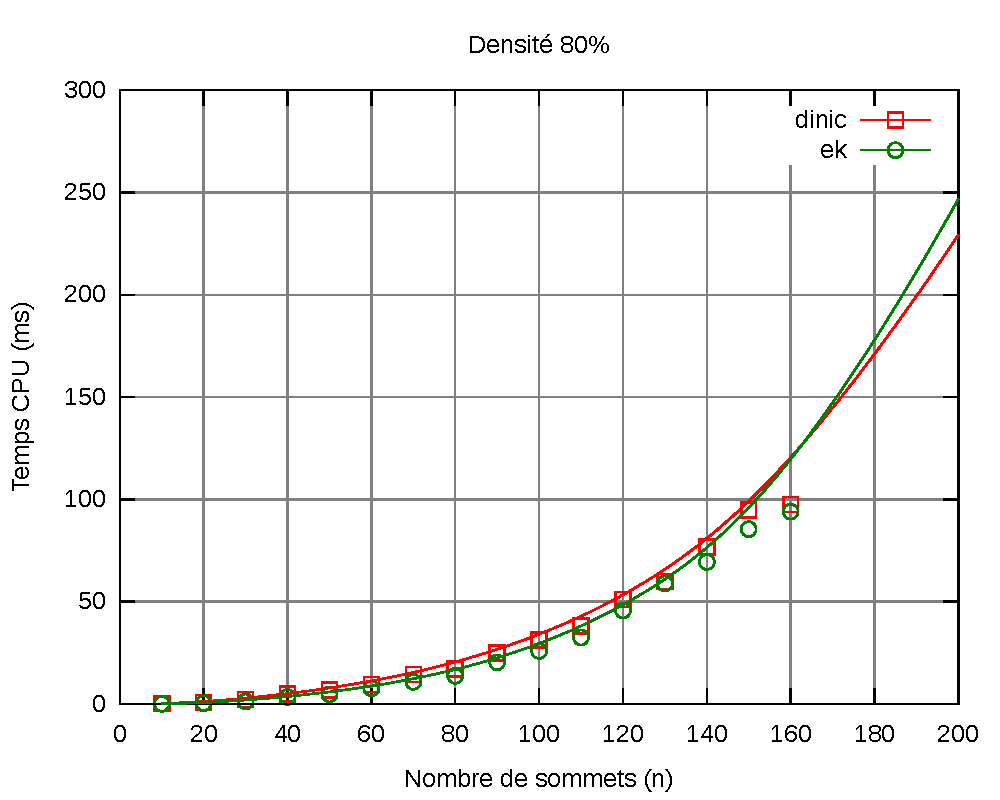
\includegraphics[width=\textwidth]{files/c80_low}
\end{center}
\caption{Temps CPU en fonction du nombre de sommets (valeur faible), densité de 80\%}
\end{figure}

On remarque ici qu'en faite, l'algorithme d'Edmonds-Karp est plus rapide que Dinic sur des graphes de 160 sommets pour une densité de 20\%, et 120 sommets pour une densité de 80\%.

De manière général, on constate que l'algorithme de Dinic est plus rapide qu'Edmonds-Karp, surtout sur des graphes peu denses. Edmonds-Karp demeure cependant plus rapide sur des graphes extrêmement petits (nombre de sommets inférieurs à 150), d'autant plus si le graphe est peu dense.